\cotefile{68}
\scanpage{45}
\uline{Prop}
$A$ $\mathbb{Q}$-alg. comm. unif.

$u$ un autom. de $\mathbb{Q}$-alg., $n\in\mathbb{N}$,
\inserted{$J$ l'idéal engendré par les $u(x)-x$ $(x\in\unsure{A|\Delta})$}

\margin{\uline{NB} $u$ induit l'identité sur $\mathrm{gr}_{J}(A)$}

1) Conditions équivalentes

(i) $u$ op. diff d'ordre $\leq n$

\margin{\deleted{\unsure{(ii$'$) $u$ induit l'identité}}}
% slanted
(ii) $J^{n+1}=0$

\margin{\deleted{(iii$'$) $\exists I$ tel que $I^{n+1}=0$, et que $u$ induise l'identité sur $\mathrm{gr}_{I}(A)$ \unsure{(ou}}}
% slanted
(iii) $\exists I$ idéal \inserted{de $A$} tel que $I^{n+1}=0$, et que $u$ induise \deleted{\unsure{la|les}} l'identité sur $A/I$, i.e.
\[
ux-x\in I\qquad \forall x\in A\qquad [\text{i.e. }I\supset J]
\]

\deleted{(iv)} Pour ceci, il \uline{suffit} que $(u-\mathrm{id})^{n+1}=0$, ou (ce qui revient au $=$)

$\exists$ dérivation $\Theta:A\longrightarrow A$ avec
\[
\Theta^{n+1}=0,\qquad u=\exp\Theta
\]
\margin{\unsure{ou bien|a-t-on|est-il} nécessaire ?}

\deleted{\uline{NB}\textsuperscript{\unsure{Si|bis}} Si $N(A)$ est nilpotent, ces conditions \unsure{équivalent|équiv.|équivalentes}}

2) L'application
\[
\Theta\longmapsto\exp\Theta
\]
est une bijection de l'ens des dérivations $\Theta$ de $A$ telles que $\Theta^{n+1}=0$, dans l'ens des autom $u$ de $A$ \inserted{telles que $(u-\mathrm{id})^{n+1}=0$ (qui} satisfaisant \inserted{donc les} conditions équivalentes plus haut).

\uline{Cor} Conditions équivalentes sur autom $u$

(i) $u$ op. diff

(ii) $J$ idéal nilp.

(iii) $\exists I$ nilp. \unsure{$\lhd A$|de $A$} tel que $u$ induise $\mathrm{id}_{A/I}$

(iv) $\exists\Theta$ dérivation nilp. \deleted{de $A$}, telle que $u=\exp\Theta$

De plus, $\Theta\unsure{\vdash|\longmapsto}\exp\Theta$ est une bij de l'ens des dérivations nilpotentes de $A$, et l'ens des autom de $A$ qui sont des op. diff.
% archive sheet number: 44
\scanpage{46}
\uline{Cor} \deleted{$A$} Supposons $NA$ nilp. \deleted{\unsure{tel}} (\unsure{p.|pr.} ex. $A$ \unsure{noth|noeth|noeth.}). Alors les conditions précédentes sur $u$ équivalent à :

(v) $u$ induit l'identité sur $A_{\mathrm{red}}$

Dans ces conditions, $\deleted{\unsure{\exists|\text{et}}}$ si \deleted{\unsure{$A$}} $N(A)^{N+1}=0$, les conditions \unsure{des|de} la prop sont satisfaites pour $(u,N)$, i.e. \unsure{tt|l'$A$|l'|$u$} opérateur diff de $A$ est d'ordre $\leq N$.

\uline{Cor.} Supposons $A$ une $K$-alg ($K$ une $\mathbb{Q}$-alg). Si $u=\exp\Theta$ ($\Theta$ dérivation nilpotente) alors $u$ est un $K$-autom \unsure{sss|ssi} $\Theta$ est une $K$-dérivation.

\uline{Cor} Soit $I$ un \unsure{idéal} nilpotent de \deleted{\unsure{$A$}}\unsure{la} $K$-alg. comm. $A$ ($K$ $\mathbb{Q}$-alg. commutative et unifère\unsure{..|...}), \inserted{$I^{N+1}=0$,} soit $L_K(A,I)$ l'ens des $K$-dérivations \deleted{de}$\Theta$ \deleted{\unsure{$A$}} de $A$ qui induisent $0$ dans $A/I$ (i.e $\Theta(A)\subset I$), $G_K(A,I)$ le groupe des $K$-autom. de $A$ \deleted{\unsure{telles|tels}} qui induisent l'identité sur $\deleted{\unsure{\Theta|0}}A/I$ (i.e. $(u-\mathrm{id})(A)\subset I$ i.e $u(x)-x\in I\quad\forall x\in A$).

Alors \quad a) $\forall\Theta\in L_K(A,I)$, on a $\Theta^{N+1}=0$

(plus généralement, $\deleted{\Theta^{i}\unsure{A}}\unsure{\forall i|i}\in\mathbb{N},\quad\Theta^i A\subset I^i$)

\[
\text{b)}\quad\Theta\longmapsto\exp\Theta:\quad L_K(A,I)\simeq G_K(A,I)
\]
% archive sheet number: 45
\scanpage{48}
\uline{Jeux à $N$ joueurs}.

$C$ ensemble des configurations (ou positions)

$J$ ensemble des joueurs \quad ($\mathrm{Card}\,J=N$)

$\underline{j}:C\unsure{-|\to}J$ \quad application \quad (pour la configuration, il y a un joueur ``dont c'est le tour'', ou concerné)

$\sigma:C\longrightarrow\mathfrak{P}(C)$ \quad pour toute configuration \inserted{$x$}, il y a l'ensemble $\sigma(x)$ des configurations ``suivantes''

\[
\unsure{\Vert|\Updownarrow}
\]
$\Sigma\subset C\times C$ \quad une relation \qquad $[$\uline{NB}. \quad $(x,y)\in\Sigma\Longleftrightarrow y\in\sigma(x)]$

$x_0\in C$ \quad configuration initiale.

$C_0\subset C$ \quad ens des configurations \deleted{\uline{gagnantes}} \uline{terminales}
\[
\text{i.e.}\qquad C_0=\{x\in C\mid\sigma(x)=\varnothing\}
\]

\deleted{Jeu} \uline{Partie} \qquad soit $j_0=\underline{j}(x_0)$ \qquad (joueur initial)

1) $j_0$ ``choisit'' un $x_1\in\sigma(x_0)$. Soit $j_1=\underline{j}(x_1)$

2) $j_1$ ``choisit'' un $x_2\in\sigma(\deleted{\unsure{j}}x_1)$ \qquad Soit $j_2=\underline{j}(x_2)$

---

$n$) $j_{n-1}$ ``choisit'' $x_{\unsure{n|n+1}}\in\sigma(\deleted{\unsure{j}}x_{n-1})$

Partie à $n$ coups :
\[
\begin{aligned}
&\deleted{\unsure{(x_0,}}(x_1,\text{---},x_n)\in C^n\\
&x_i\in\sigma(x_{i-1})\qquad 1\leq i\leq n
\end{aligned}
\]

\uline{Jeu circulaire} \qquad 1) $j$ surjectif (tout joueur est effectif)

2) $\exists\deleted{\unsure{x}}\ \rho:J\longrightarrow J$ telle que
\[
\begin{aligned}
&\deleted{\forall x\in C,\ y\in\sigma(x)}\\
&\forall(x,y)\in\Sigma\subset C\times C,\text{ on a }\ j(y)=\rho(j(x))
\end{aligned}
\]

\uline{NB} $\rho$ unique si on suppose que $\forall x\in C$, \inserted{\unsure{on a}} $\sigma(x)\neq\varnothing$, ou plus gén. que $\forall j\in J$, $\exists x\in C$ tel que $\sigma(x)\neq\varnothing$, $\underline{j}(x)=j$

3) $\rho$ est une permutation circ.
% archive sheet number: 47
\scanpage{50}
\uline{Lemme 1} \quad $P,Q$ ens. de card. $2$, \inserted{$x\in P$ \deleted{\unsure{unique|x'}} $x'=\underline a_P x$} $\varphi:P\to Q$ conditions équivalentes

a) $\varphi$ bij \qquad b) $\varphi$ inj \qquad c) $\varphi$ surj \qquad d) $\varphi$ non constante

e) $\varphi$ commute à $\mathbb{Z}_2$ \qquad f) $\varphi(x')=\underline a_Q\varphi(x)$

\uline{Lemme 2} \quad $P,Q,R$ ens. de card. $2$, $\varphi:P\times Q\unsure{-|\to}R$ app., $x\in P$, $x'=\underline a x$

Conditions équivalentes

a) $\varphi$ se factorise en iso \qquad $P\wedge Q\to R$

b) $\varphi_x:y\unsure{\leftrightarrow|\mapsto}\varphi(x,y):Q\to R$ est iso, et $\varphi_{x'}\deleted{\unsure{=\varphi_x|\varphi_x}}=\underline a_R\varphi_x$

Théorie orientation pour vectoriels réels de dim finie (cat. $\mathcal V\deleted{\unsure{f}}$, avec \uline{iso})

a) $\deleted{\unsure{\forall V\in\mathrm{Ob}\,\mathcal V}}$\qquad $\Omega:\mathcal V\longrightarrow(\mathrm{Ens})$

b) $\Omega(0)\simeq\{\pm1\}$

c) $\forall V\in\mathrm{Ob}\,\mathcal V$, \deleted{\unsure{un}} $W\subset V$ hyperplan, $V'$ demi-espace de $V$ de frontière $W$, on donne application de Stokes
\[
\mathrm{St}_{V'}:\Omega(V)\longrightarrow\Omega(W)\qquad\text{\uline{fonctoriel} \uline{en} }(V,V')
\]

\uline{Axiomes} \qquad 1) $\mathrm{St}_{V'}$ bijectif \deleted{(cf \unsure{lemme 1})}\qquad \uline{Cor} $\forall V\in\mathrm{Ob}\,\mathcal V$, $\mathrm{Card}\,\Omega(\unsure{W|V})=2$

2) Si $V''$ est l'opposé de $V'$, on a $\mathrm{St}_{V''}=\underline a\circ\mathrm{St}_{V}$

\uline{Axiomes équivalents} \qquad 1) $\forall V\in\mathrm{Ob}\,\mathcal V$, $\mathrm{card}\,\Omega(V)=2$

2) $\forall V\in\mathrm{Ob}\,\mathcal V$, $W\in\mathrm{Hyp}(V)$, \deleted{2)} l'application \deleted{\unsure{demi-esp. $V$|$\Omega(W,V)$}}\inserted{$\Omega(W\unsure{/|,}V)$} $\times\Omega(V)\longrightarrow\Omega(W)$
\[
(V',\omega)\longrightarrow\mathrm{St}_{V'}(\omega)
\]
se factorise en un \deleted{application}\inserted{iso}
\[
\deleted{\unsure{\Omega_{W,V}}}\quad\Omega(W,V)\wedge\Omega(V)\xrightarrow{\sim}\Omega(W)\quad\searrow\ \text{fonctoriel en }(V,W)
\]

\deleted{\unsure{Morphisme|Proposition}} Hom d'une théorie $(\Omega,\mathrm{St})$ dans \unsure{théorie} $(\Omega',\mathrm{St}')$

hom de foncteurs $\varphi:\Omega\longrightarrow\Omega'$ compatible avec b), et c)

\uline{Th.} \deleted{\unsure{$\exists$}} a) \deleted{\unsure{Tout|tout}} hom d'une théorie dans une autre est un isom.

b) Pour 2 théories de l'orientation, $\exists!$ isom de l'une dans l'autre

c) $\exists$ théorie de l'orientation.

\uline{Dém}

a) $\varphi_V:\Omega(\unsure{W|V})\unsure{\simeq|\xrightarrow{\sim}}\Omega'(W)$ iso, par réc sur dim. utilisant Stokes

\deleted{\unsure{b) c)|b)}} De $=$, unicité de $\varphi$ par récurrence sur dim. Existence \inserted{\unsure{de $\varphi$ ?|déjà ?}}

\deleted{Détermination d'une thé} Existence d'une théorie de l'orientation ?

donner $\Omega:$\inserted{$\mathcal V\unsure{-|\to}\mathrm{Ens}_2$} $\Longleftrightarrow$ donner $(\Omega_n)_{n\in\mathbb{N}}$, $\Omega_n:\mathcal V_n\longrightarrow\mathrm{Ens}_2\deleted{\unsure{=}}\mathrm{Tors}(\mathbb{Z}_{/2})$

donner $\Omega_n\Longleftrightarrow$ donner $\varepsilon_n:\underset{\substack{\Vert\\G_n}}{\unsure{\mathrm{Gl}|\mathrm{GL}}(n,\mathbb{R})}\longrightarrow\mathbb{Z}/2$, \uline{et} $\omega_n=\Omega(\mathbb{R}^n)$

donner $\mathrm{St}\Longleftrightarrow(\mathrm{St}_n)_{n\in\mathbb{N}^{*}}$, où $\mathrm{St}_n$ est donnée de Stokes en dim $n$
\[
\Omega(V,W)\wedge\Omega(V)\unsure{\to|\ni|\xrightarrow{\sim}}\Omega(W)\qquad\text{pour }\dim V=n
\]
donner $\{\mathrm{St}_n\}_{\unsure{n\in{}|n}}$ revient à \unsure{se} donner
% archive sheet number: 49
\scanpage{51}
XVIII \qquad L\,e\,s \quad é\,p\,o\,u\,s\,a\,i\,l\,l\,e\,s \qquad (2)

J'ai scruté et j'ai fouillé - par pleines brassées je ramasse tout à l'entour les paires enlacées disant un même message. Pêle-mêle je les jette devant moi ...

Puis, comme un enfant appliqué intensément enfile collier de pierres multicolores qu'il assem\deleted{\unsure{m|n}}ble à son gré - sans en laisser une seule, car toutes lui semblent belles ! \unsure{...|-..} lestement passant les unes, et sur d'autres s'arrêtant longement pour les contempler à loisir ... ainsi du chaos chatoyant de mes trouvailles je prépare ce collier - m\,o\,n collier - pour te l'offrir ... et \deleted{pour} l'oublier ...

Le jeu était p\,l\,a\,i\,s\,i\,r - il était découverte ! Qu'importe s'il reste \deleted{\unsure{collier}}\handwritten{trace} pour témoigner du jeu \inserted{\handwritten{révolu}} d'un enfant qui découvre \deleted{\unsure{?}}\handwritten{!} Quel sens a un collier, si ce n'est le plaisir de le faire ...

Ou \unsure{...|.-.} susciter en \uline{toi} d\,é\,s\,i\,r de scruter et fouiller - de ramasser toi-même perles et pierres par poignées ... contempler longuement une à une celles qui t\,e parlent, et au gré de \deleted{\unsure{ta|la}} \uline{t\deleted{\unsure{out|ou}}\handwritten{on}}\deleted{\unsure{e|te}} d\deleted{\unsure{ernière}}\handwritten{ésir}\deleted{\unsure{ère|es}} \deleted{\unsure{à toi|fantaisie}} assembler t\,o\,n collier ?

\deleted{A quoi bon un collier qui ne suscite désir d'en faire un plus beau ?}

Je termine d'un deuxième rang de \deleted{\unsure{perles|peres}}paires enlacées \unsure{...} \deleted{s}\handwritten{S}i le jeu \deleted{\unsure{t}}\handwritten{t}e plait encore, \deleted{tu peux} regarde\deleted{r} faire ... ou \deleted{tu peux} fai\deleted{re}\handwritten{s} \deleted{\unsure{le tien|ton}}\handwritten{en un plus} \inserted{\handwritten{beau\unsure{!|.}}}

11. En les choses de la Création s'enlacent et s'unissent :

l\,u\,m\,i\,è\,r\,e \quad et \quad o\,m\,b\,r\,e\\
le clair \quad et l'obscur\\
le jour \quad et la nuit\\
le brillant \quad et le terne

savoir \quad et mystère\\
le connu \quad et l'inconnu\\
le connaissable \quad et l'inconnaissable\\
connaissance \quad et ignorance

le précis \quad et le vague\\
le particulier \quad et le général

\noindent\begin{tabular}{@{}p{.49\linewidth}@{\quad}p{.45\linewidth}@{}}
le défini \quad et l'indéfini & \makebox[0pt][r]{\smash{\begin{tikzpicture}[x=1em,y=1ex,baseline=0pt]\draw (-1.0,-11)--(.45,2.1);\end{tikzpicture}}\hspace{.35em}}nécessité \quad et hasard\\
l'exprimé \quad et l'inexprimé & veille \quad et sommeil\\[.5em]
l'achevé \quad et l'inachevé & ce qui naît - et ce qui l'enfante\\
le formé \quad et l'informe & \\
simplicité \quad et complexité & ce qui meurt - et ce qui l'accueille\\
ordre \quad et chaos &
\end{tabular}
% archive sheet number: 50
\scanpage{52}
\[
\underbrace{\Omega(\mathbb R^{n-1},\mathbb R^{\unsure{+n|n}})}_{1}\wedge\Omega(\mathbb R^n)\longrightarrow\Omega(\mathbb R^{n-1})\qquad\text{i.e.}
\]
\margin{on choisit $\mathbb R^{n-1}\times\mathbb R^{+}$ comme $1/2$ espace de $\mathbb R^n$}
\[
-\ \omega_n\xrightarrow{\sim}\omega_{n-1}
\]
compatible avec $\mathrm{Aut}(\mathbb R^{n-1},\mathbb R^n)={}$ \unsure{ssgrpe|ss-gr.} de $\mathrm{Gl}(n,\mathbb R)$ des matrices
\[
u_n=\deleted{\left(\overbrace{\underline{\quad\unsure{u}\quad}}^{n-1}\right|}
\left(\begin{array}{c@{\;}c|c}
&\overbrace{\hphantom{u_{n-1}}}^{n-1}&\unsure{?|a|0}\\[-1ex]
\scriptstyle n-1\big\{&u_{n-1}&\vdots\\
&&\unsure{?|b|0}\\[-.5ex]\cline{2-2}
&0\qquad 0&\lambda
\end{array}\right)
\]
opérant sur $\omega_{n-1}$ par $\deleted{\unsure{\mathrm{sg}\,\det|\varepsilon}}\varepsilon_{n-1}(u_{n-1})$, sur $\omega_n$ par $\deleted{\unsure{\mathrm{sg}\,\det}}\inserted{\varepsilon_n}(u_n)\cdot\mathrm{sg}\,\lambda$ \deleted{\unsure{$=$, égalité qui se traduit|$\mathrm{sg}\,\det$}} \inserted{condition qui \unsure{s'exprime|signifie}}
\[
\deleted{\unsure{\det u_{n-1}}}\qquad
\boxed{\varepsilon_n(u_n)=\mathrm{sg}(\lambda)\varepsilon_{n-1}(u_{n-1})}.
\]

\deleted{qui est donc \unsure{automatiquement} satisfaite !}

\deleted{Donc la donnée d'une théorie \unsure{des Or.|de l'or.|de l'orient.} s'identifie à la donnée de $\{(\varepsilon_n)\}_{n\in\mathbb N}$, où $\varepsilon_n:G_n\longrightarrow\{\pm1\}$ \par $\unsure{(\varepsilon_n)_{n\in\mathbb N^*}}\quad\text{où}\quad\unsure{\varepsilon_n|s}:\omega_n\xrightarrow{\sim}\omega_{n-1}$ \par car les $\omega_n\simeq\omega_{n-1}$, et $\omega_0\simeq\{\pm1\}$, donnent $\omega_n\simeq\{\pm1\}$.}

Ceci détermine $\varepsilon_1:\mathbb R^*\longrightarrow\{\pm1\}$ par
\[
\varepsilon_1=\mathrm{sg}:\mathbb R^{\unsure{+|*}}\unsure{-|\to}\{\pm1\}
\]
et \unsure{je dis|pr des|de proche} plus gén, par récurrence
\[
\varepsilon_n(u)=\mathrm{sg}\circ\det(u)\qquad u\in\mathrm{Gl}(n,\mathbb R)
\]

\deleted{\unsure{\illegible{1}|Lemme 2}}\qquad $=$
% archive sheet number: 51
\scanpage{53}
\mspage{\handwritten{82}}

XVIII \quad L\,e\,s \quad é\,p\,o\,u\,s\,a\,i\,l\,l\,e\,s \qquad (2)

J'ai scruté et j'ai fouillé - par pleines brassées je ramasse tout à l'entour les paires enlacées disant un même message. Pêle-mêle je les jette devant moi ...

Puis, comme un enfant appliqué intensément enfile collier de pierres multicolores qu'il assemmble à son gré - sans en laisser une seule, car toutes lui semblent belles !\unsure{...|--} lestement passant les unes, et sur d'autres s'arrêtant longement pour les contempler à loisir ... ainsi du chaos chatoyant de mes trouvailles je prépare ce collier - m\,o\,n collier - pour te l'offrir ... et \deleted{pour} l'oublier ...

Le jeu était p\,l\,a\,i\,s\,i\,r - il était découverte ! Qu'importe s'il reste \deleted{collier}\handwritten{trace} pour témoigner du jeu \inserted{\handwritten{révolu}} d'un enfant qui découvre \unsure{?|!} Quel sens a un collier, si ce n'est le plaisir de le faire ...

Ou ... susciter en \uline{toi} \deleted{\unsure{des|le}}d\handwritten{é}\unsure{s}\handwritten{i}\unsure{r}\deleted{\unsure{vie|une}} de scruter et fouiller - de ramasser toi-même perles et pierres par poignées ... contempler longuement une à une celles qui t\,e parlent, et au gré de \deleted{ta} \uline{to\handwritten{n}}\deleted{\unsure{te|e}} \deleted{\unsure{dernièr|désir}}\inserted{\handwritten{désir}} \deleted{\unsure{à toi|à quoi|enant}} assembler t\,o\,n collier ?\margin{\handwritten{[}}

\deleted{A quoi bon un collier qui ne suscite désir d'en faire un plus beau ?}

\margin{\handwritten{[}}Je termine d'un deuxième rang de \deleted{\unsure{perles|peres}}paires enlacées\unsure{...|.} \handwritten{S}i le jeu te plait encore, \deleted{tu peux} regarde\deleted{r} faire - ou \deleted{tu peux} fai\deleted{\unsure{r|re}}\handwritten{s}\deleted{\unsure{e}}-\handwritten{en} \deleted{\unsure{ton|le|toi} \unsure{jeu|tien|à toi}}\inserted{\handwritten{un plus beau !}}

11. En les choses de la Création s'enlacent et s'unissent :

\begin{tabular}{@{}l@{}}
l\,u\,m\,i\,è\,r\,e \quad et \quad o\,m\,b\,r\,e\\
le clair \quad et l'obscur\\
le jour \quad et la nuit\\
le brillant \quad et le terne\\[.6ex]
savoir \quad et mystère\\
le connu \quad et l'inconnu\\
le connaissable \quad et l'inconnaissable\\
connaissance \quad et ignorance\\[.6ex]
le précis \quad et le vague
\end{tabular}

\begin{tabular}{@{}p{.48\linewidth}@{\quad}p{.43\linewidth}@{}}
le particulier \quad et le général & \\
le défini \quad et l'indéfini & \makebox[0pt][r]{\smash{\begin{tikzpicture}[x=1em,y=1ex,baseline=0pt]\draw (-1.0,-11)--(.45,2.1);\end{tikzpicture}}\hspace{.35em}}nécessité \quad et hasard\\
l'exprimé \quad et l'inexprimé & veille \quad et sommeil\\[.6ex]
l'achevé \quad et l'inachevé & ce qui naît - et ce qui l'enfante\\
le formé \quad et l'informe & ce qui meurt - et ce qui l'accueille\\
simplicité \quad et complexité &\\
ordre \quad et chaos &
\end{tabular}

% archive sheet number: 52
\scanpage{54}
\[
U\underset{\omega'}{\underbrace{\subset}}W\underset{\omega}{\underbrace{\subset}}V
\qquad
\Omega(V/W)\wedge\Omega(V)\longrightarrow\Omega\unsure{W)|(W)}
\]

\[
\begin{aligned}
\mathrm{St}_{\omega}:&\ \Omega(V)\unsure{\longrightarrow|-}\Omega W)\\
\mathrm{St}_{\omega'}:&\ \Omega(W)-\Omega(U)
\end{aligned}
\]
\[
\mathrm{St}_{\omega'}\mathrm{St}_{\omega}:\quad \Omega(V)\longrightarrow\Omega(U)
\]
\[
I(\omega,\omega')\in\Omega
\]

\margin{$(\omega,\omega')\unsure{\mapsto|\vdash}\omega\times\omega'$}
\[
\Omega\unsure{(V)|(W)}\wedge\Omega\unsure{(V')|(W')}\longrightarrow\Omega(V\wedge V')
\]
\[
\omega'\times\omega=(-1)^{\dim V\cdot\dim V'}\deleted{\unsure{\Omega V'|\Omega V}}\ \omega\times\omega'
\]

$\deleted{\mathrm{St}(\omega)\,\mathrm{St}(\omega')}$

\diagram{$\begin{array}{c@{}c@{}c@{}c@{}c@{\quad}c@{\quad}c@{}c@{}c}
\mathbb R&\subset&\mathbb R^2&\subset&\mathbb R^3&-&\mathbb R^{n-1}&\subset&\mathbb R^n\\[-.4ex]
\unsure{\cup|\vee}&&\cup&&\cup&&\cup&&\cup\\[-.4ex]
R^+&\subset&\mathbb R\times\mathbb R^+&\subset&\mathbb R^2\times\mathbb R^+&\subset&
\mathbb R^{\unsure{n-2}}\times\mathbb R^+&\subset&\mathbb R^{n-1}\times\mathbb R^+
\end{array}$}
\[
\unsure{e|a}_1\wedge\cdots e_{n-1}\wedge e_n
\qquad
e_1\wedge\cdots\wedge e_{n-1}\wedge e_n
\]
\[
\omega\times\omega'\qquad I(\omega,\omega')\qquad I(\omega',\omega)
\]

\[
\left\{\begin{aligned}
\mathrm{St}(\omega\times\omega')&=\inserted{(-1)^{\unsure{q|?}}}\mathrm{St}(\omega)\times\omega'\\
\mathrm{St}(\omega\unsure{,|\times}\omega')&=\deleted{\unsure{(-1)^q}}\omega\times\mathrm{St}\,\omega'
\end{aligned}\right.
\]
\[
\underbrace{e_1\cdots e_p}\quad f_1\cdots f_q
\]
\[
\unsure{\mathrm{St}|M}(e_1\cdots e_{p-1}\,e_p\,f_1\cdots f_q)=(-1)^{\unsure{q|1}}
\unsure{(e_1|e_1}\cdots e_{p-1}\,\widehat e_p\,f_1\cdots\unsure{f_q|f_2}
\]
\[
e_1\ e_2\cdots e_n
\]

\figure{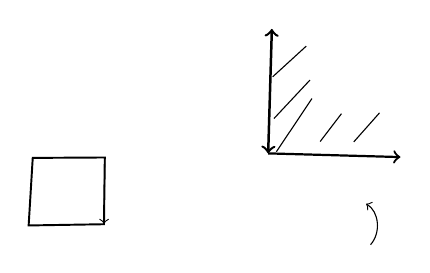
\begin{tikzpicture}[x=.52cm,y=.52cm]
\draw[line width=.7pt] (0,0)--(.10,1.65)--(1.86,1.66)--(1.84,.03)--cycle;
\draw[->] (1.86,1.62)--(1.84,.04);
\draw[<->,line width=.9pt] (5.85,1.76)--(5.94,4.80);
\draw[->,line width=.8pt] (5.85,1.76)--(9.08,1.67);
\draw[thin] (5.96,3.63)--(6.78,4.38) (5.99,2.61)--(6.87,3.55)
 (6.05,1.80)--(6.92,3.10) (7.12,2.05)--(7.64,2.73) (7.94,2.04)--(8.57,2.75);
\draw[->] (8.35,-.47) .. controls (8.61,-.18) and (8.56,.34) .. (8.24,.53);
\end{tikzpicture}}

% archive sheet number: 53
\scanpage{55}
XVIII \quad L\,e\,s \quad é\,p\,o\,u\,s\,a\,i\,l\,l\,e\,s \qquad (2)

J'ai scruté et j'ai fouillé - par pleines brassées je ramasse tout à l'entour les paires enlacées disant un même message. Pêle-mêle je les jette devant moi ...

Puis, comme un enfant appliqué intensément enfile collier de pierres multicolores qu'il assem\deleted{\unsure{m|n}}ble à son gré - sans en laisser une seule, car toutes lui semblent belles ! \unsure{...|--.} lestement passant les unes, et sur d'autres s'arrêtant longement pour les contempler à loisir ... ainsi du chaos chatoyant de mes trouvailles je prépare ce collier - m\,o\,n collier - pour te l'offrir ... et \deleted{pour} l'oublier ...

Le jeu était p\,l\,a\,i\,s\,i\,r - il était découverte ! Qu'importe s'il reste \deleted{\unsure{collier}}\handwritten{trace} pour témoigner du jeu \inserted{\handwritten{révolu}} d'un enfant qui découvre \unsure{?|!} Quel sens a un collier, si ce n'est le plaisir de le faire ...

Ou \unsure{...|.-.} susciter en \uline{toi} d\,é\,s\,i\,r de scruter et fouiller - de ramasser toi-même perles et pierres par poignées ... contempler longuement une à une celles qui t\,e parlent, et au gré de \deleted{ta} \uline{t\deleted{\unsure{out|ou}}\handwritten{on}}\deleted{\unsure{e|te}} d\deleted{\unsure{ernière|ernier}}\handwritten{ésir}\deleted{\unsure{ère|es}} \deleted{\unsure{à toi|fantaisie}} assembler t\,o\,n collier ?

\deleted{A quoi bon un collier qui ne suscite désir d'en faire un plus beau ?}

Je termine d'un deuxième rang de \deleted{\unsure{perles|peres}}paires enlacées \unsure{...|.--} \deleted{s}\handwritten{S}i le jeu \deleted{\unsure{t|d}}\handwritten{t}e plait encore, \deleted{tu peux} regarde\deleted{r} faire ... ou \deleted{tu peux} fai\deleted{re}\handwritten{s} \deleted{\unsure{le|ton|toi}}\handwritten{en} \deleted{\unsure{tien|un|jeu}}\handwritten{un plus} \inserted{\handwritten{beau!}}

11. En les choses de la Création s'enlacent et s'unissent :

\begin{tabular}{@{}l@{}}
l\,u\,m\,i\,è\,r\,e \quad et \quad o\,m\,b\,r\,e\\
le clair \quad et l'obscur\\
le jour \quad et la nuit\\
le brillant \quad et le terne\\[.6ex]
savoir \quad et mystère\\
le connu \quad et l'inconnu\\
le connaissable \quad et l'inconnaissable\\
connaissance \quad et ignorance\\[.6ex]
le précis \quad et le vague
\end{tabular}

\begin{tabular}{@{}p{.48\linewidth}@{\quad}p{.43\linewidth}@{}}
le particulier \quad et le général &\\
le défini \quad et l'indéfini & \makebox[0pt][r]{\smash{\begin{tikzpicture}[x=1em,y=1ex,baseline=0pt]\draw (-1.0,-11)--(.45,2.1);\end{tikzpicture}}\hspace{.35em}}nécessité \quad et hasard\\
l'exprimé \quad et l'inexprimé & veille \quad et sommeil\\[.6ex]
l'achevé \quad et l'inachevé & ce qui naît - et ce qui l'enfante\\
le formé \quad et l'informe & ce qui meurt - et ce qui l'accueille\\
simplicité \quad et complexité &\\
ordre \quad et chaos &
\end{tabular}

% archive sheet number: 54
\scanpage{56}
$k$ \unsure{anneau} comm.

$\unsure{\mathcal V|\mathscr V}=\mathcal V(k)$ catégorie des modules libres de type fini sur $k$ (morphismes : \uline{iso})
\[
\overset{\text{\textquotedbl}}{\coprod_{n\in N}}\mathcal V_n(k)\qquad \mathcal V_n(k)\ \text{catégorie des modules libres de rang }n\text{ sur }k
\]
$\mathcal V$ catégorie additive (\unsure{graduée|gr. duée})

\deleted{\unsure{a)} $\mathcal V\xrightarrow{\Delta}\mathcal V_{\unsure{1|\mathbb Z}}$ foncteur}

\deleted{\unsure{b)} $\unsure{\mathcal V}$.} $\mathcal P(k)$ catégorie de Picard des $k$-modules libres de rang $1$ $Z$-gradués, avec donnée de comm. l'isomorphisme de \unsure{Koszul|Koszuel}

\uline{Théorie des \inserted{modules} \unsure{déterminantiels|déterminants|déterminant} gradués}

a) $\mathcal V\xrightarrow{\Delta}\mathcal P$ \quad $\otimes$ foncteur (donc muni d'iso fonct.
\[
\Delta(V+V')\overset{\varphi_{V,V'}}{\simeq}\Delta(V)\otimes\Delta(V')
\]
\margin{\deleted{\unsure{gr|g}}}
\[
(\Rightarrow\Delta(0)\simeq\underline{1}\quad\text{can}^{\unsure{\mathrm t|\mathrm l}})
\]

b)\deleted{\unsure{a)}} Si $\mathrm{rg}(V)=1$, \quad $\Delta(V)\simeq V$, de degré $1$

c) Soient $V\supset W_1$, $W_2,W'_2$ deux suppl. de $W_1$ dans $V$ ($W_1,W_2$ libres dans $V$, $W'_2$ \unsure{aussi|ni}).
\[
\begin{aligned}
\alpha &: W_1+W_2\xrightarrow{\sim} V\\
\alpha' &: W_1+W'_2\xrightarrow{\sim} V\\
\lambda &: W_2\simeq W'_2
\end{aligned}
\]

\diagram{\begin{tikzcd}[ampersand replacement=\&,column sep=1.5em,row sep=3.6em]
\Delta(W_1+W_2) \arrow[r,"{\substack{\Delta(\alpha)\\ \sim}}"] \arrow[d,no head,"{\rotatebox{90}{$\sim$}\ \varphi_{\unsure{W_1,W_2)|W_1,W_1)}}}"]
\& \Delta(\unsure{W|V})
\& \Delta(W_1+W'_2) \arrow[l,"{\substack{\Delta(\alpha')\\ \sim}}"'] \arrow[d,no head,"{\rotatebox{90}{$\sim$}\ \varphi_{W_1,W'_2}}"]\\
\Delta(V_1)\otimes\Delta(W_2)
\& \& \Delta(W_1)\otimes\Delta(W'_2) \arrow[ll,"{\substack{\mathrm{id}\otimes\Delta(\lambda)\\ \sim}}"']
\end{tikzcd}}

commutatif.

[ \unsure{Équivaut|Equivaut} à : Si $u$ est un \unsure{autom.|automorph.} de $V$ qui est l'identité sur $W_1$ et sur $V/W_1$ ($\simeq W_2^{\unsure{\prime|\cdot|{}}}$), alors $\Delta(u)=\mathrm{id}_{\Delta(V)}$ ]
% archive sheet number: 55
